%*******10********20********30********40********50********60********70********80
%% ----------------------------------------------------------------
%% Thesis.tex -- MAIN FILE (the one that you compile with LaTeX)
	%% ---------------------------------------------------------------- 

%% This template is based on Graduate Thesis written by Sunil Patel,
% (ho based it on the ecsthesis template) under the LaTeX Project Public License.
% which can be found here: http://latex-project.org/lppl/
% in the hope that it will be easier to use and to scale down to your needs
% by Simon Ternsjö in 2013-10



% INSTRUCTIONS:

% The meaning is not to edit this document much, but to fill in information 
% in the different files in the folders;
% Settings, Frontpages, Chapters, Appendices and possibly Files,
% as well as the file Bibliography.bib

% This template is easy to scale down to suite your need, 
% simply comment the input statements explained below


% Set up the document:
\documentclass[a4paper, 11pt, oneside]{Thesis}  % Use the "Thesis" style, based on the ECS Thesis style by Steve Gunn

% Add more package in Package.tex:
% Add your own packages here, 
% these existing packages can be removed if necessary
% not that more packages are imported in Thesis.cls, '
%  but those should not be changed if you don't know what you are doing...


\usepackage[utf8]{inputenc} % for writing other that basic characters
\usepackage{graphicx}
\usepackage{caption}
\usepackage{subcaption}
\usepackage{media9}


% Include any extra LaTeX packages required
\usepackage[square, numbers, comma, sort&compress]{natbib}  % Use the "Natbib" style for the references in the Bibliography
\usepackage{verbatim}  % Needed for the "comment" environment to make LaTeX comments
%5%\usepackage{vector}  % Allows "\bvec{}" and "\buvec{}" for "blackboard" style bold vectors in maths




% Use if you want:
%5%\graphicspath{Figures/}  % Location of the graphics files (set up for graphics to be in PDF format)
%5%\hypersetup{urlcolor=blue, colorlinks=true}  % Colours hyperlinks in blue, but this can be distracting if there are many links.

% Set your name, the title of the report and more in Administraitve.tex:
% This is where author, university, title and more is defined

% Personal information:
\newcommand{\myAuthorName}  {Mridul Birla}% Author Name
\newcommand{\myAuthorEmail} {mbirla@iu.edu} % Author email
\newcommand{\myTitle}       {Improved Conditional Adversarial Network} % Thesis title goes here
\newcommand{\mySubject}     {} % Subject goes here
\newcommand{\myKeywords}    {Computer Vision, CNN, GAN} % Keywords goes hear




% University information
\newcommand{\myUniversity}{Indiana University Bloomington} %The Iniversity name goes here
\newcommand{\myUniversityWeb}{https://www.indiana.edu/} %University Web Site URL Here (include http://
\newcommand{\myDepartment}{SCHOOL OF INFORMATICS AND COMPUTING} % The Department goes here 
\newcommand{\myDepartmentWeb}{http://www.soic.indiana.edu/} % Department Web Site URL Here (include http://)

%Degree, program or corse: ex: Master of Science, Engineering Physics
\newcommand{\myDegree}{Master of Science} % The degree, program or course-name goes here


% can be left untouched, both:
\newcommand{\myDate}{\today}
\newcommand{\myPartyalFulfillment}{A thesis submitted in partial fulfillment for the degree of}

%% ----------------------------------------------------------------
\begin{document}
\frontmatter      % Begin Roman style (i, ii, iii, iv...) page numbering


% Here the first pages are imported, you can find them in the Frontpages folder
% Files in the subfolder Fixed does not need to be edited.
% If you don't need any of these sections, simply comment, or delete, the input-row


%% All the pages before the chapters ------------------------------
% Set up the Title Page - DO NOT EDIT THIS, (if you don't want to ;)  )
% instead specify your name, title and more in "/Settings/Administrative.tex"
\title   {\myTitle}
\authors {\texorpdfstring
            {\href{\myAuthorEmail}{\myAuthorName}}
            {\myAuthorName}
         }
\addresses  {\groupname\\\deptname\\\univname}  
\date       {\myDate}
\subject    {\mySubject}
\keywords   {\myKeywords}

\maketitle
%% ----------------------------------------------------------------

\setstretch{1.3}  % It is better to have smaller font and larger line spacing than the other way round

% Define the page headers using the FancyHdr package and set up for one-sided printing
\fancyhead{}  % Clears all page headers and footers
\rhead{\thepage}  % Sets the right side header to show the page number
\lhead{}  % Clears the left side page header


%% ----------------------------------------------------------------
% Declaration Page required for the Thesis, your institution may give you a different text to place here
\pagestyle{fancy}  % Finally, implement the FancyHdr headers
\clearpage
\Declaration{

\addtocontents{toc}{\vspace{1em}}  % Add a gap in the Contents, for aesthetics

I, \myAuthorName, declare that this thesis titled, `\myTitle' and the work presented in it are my own. I confirm that:

\begin{itemize} 
\item[\tiny{$\blacksquare$}] This work was done wholly or mainly while in candidature for a research degree at this University.
 
\item[\tiny{$\blacksquare$}] Where any part of this thesis has previously been submitted for a degree or any other qualification at this University or any other institution, this has been clearly stated.
 
\item[\tiny{$\blacksquare$}] Where I have consulted the published work of others, this is always clearly attributed.
 
\item[\tiny{$\blacksquare$}] Where I have quoted from the work of others, the source is always given. With the exception of such quotations, this thesis is entirely my own work.
 
\item[\tiny{$\blacksquare$}] I have acknowledged all main sources of help.
 
\item[\tiny{$\blacksquare$}] Where the thesis is based on work done by myself jointly with others, I have made clear exactly what was done by others and what I have contributed myself.

\end{itemize}
 
\vspace{10 mm}
 
Signed:\\
\rule[1em]{25em}{0.5pt}  % This prints a line for the signature

Date:\\
\rule[1em]{25em}{0.5pt}  % This prints a line to write the date
}



% The "Funny Quote Page"
\clearpage
\pagestyle{empty}  % No headers or footers for the following pages

%use 1 or vfill to position the quote where it looks good:
\null\vfill\vfill


% Now comes the "Funny Quote", written in italics:

\textit{
    % Write a funny quote here:
    ''We did it, we bashed them, wee Potter’s the one, \\
    and Voldy’s gone moldy, so now let’s have fun!''
}
\begin{flushright}
    % If the quote is taken from someone, their name goes here:
    - Peeves
\end{flushright}


 
\vfill\vfill\vfill\vfill\vfill\null


% The Abstract Page
\clearpage 
\addtotoc{Abstract}  % Add the "Abstract" page entry to the Contents     
\abstract{
    \addtocontents{toc}{\vspace{1em}}  % Add a gap in the Contents, 
                                        %for aesthetics
    
    %The Thesis Abstract is written here (and usually kept to just this page). 
    %The page is kept centered vertically so can expand into the blank space above the title too \ldots
    
    Any complex computer vision problems have now become approachable with the advancements in the areas of deep learning. Generative neural network frameworks have been one of the most recent developments in this field. These networks have shown promising results of generating real world synthetic images such as of bedrooms, cats, human faces etc. These frameworks are being applied to various computer vision applications and once such challenging problem is generating images. In this work, we scrutinize various generative frameworks such as Deep Convolution Generative Adversarial Network(DCGAN),, InfoGAN. We then, train the a improved generative network

    
}



% The Acknowledgements page, for thanking everyone
\clearpage
\setstretch{1.3} % Reset the line-spacing to 1.3 for body text (if changed)
\acknowledgements{
    \addtocontents{toc}{\vspace{1em}} %Add a gap in the Contents, for aesthetic
    
    % The acknowledgements and the people to thank go here, don't forget to include your project advisor...
    
    % The following are examples of how to word your thanks
    
    I would like to express my very great appreciation to Susan Bones 
    for the \ldots
    
    I would also like to offer my special thanks to Cedric Diggory 
    for\ldots
    
    My special thanks are extended to the staff of the Matron
    for\ldots
    
    My special thanks goes to Pomona Sprout for taking on this thesis work.
    
    I am particularly grateful for the support and good times given by my friends, 
    for\ldots
    
    To my family, for\ldots, 
    I am particularly grateful.
    
    Advice given by Helga Hufflepuff has been a great help in\ldots
    
    To my beloved Ernie Macmillan for all the\ldots
}


\clearpage
\setstretch{1.3} % Reset the line-spacing to 1.3 for body text (if changed)
\pagestyle{fancy} % The page style headers have been "empty" all this time, 
                  % now use the "fancy" headers as defined before
\lhead{\emph{Contents}}  % Set the left side page header to "Contents"
\tableofcontents  % Write out the Table of Contents


\setstretch{1.3} % Reset the line-spacing to 1.3 for body text (if changed)
\pagestyle{fancy} % The page style headers have been "empty" all this time, 
                  % now use the "fancy" headers as defined before
\lhead{\emph{List of Figures}}  % left side page header to "List if Figures"
\listoffigures  % Write out the List of Figures


\clearpage  % Start a new page
\setstretch{1.3} % Reset the line-spacing to 1.3 for body text (if changed)
\pagestyle{fancy} % The page style headers have been "empty" all this time, 
                  % now use the "fancy" headers as defined before
\lhead{\emph{List of Tables}}  % left side page header to "List of Tables"
\listoftables  % Write out the List of Tables


\clearpage
\pagestyle{fancy} % The page style headers have been "empty" all this time, 
                  % now use the "fancy" headers as defined before
\setstretch{1.5} % Set the line spacing to 1.5, 
                 % this makes the following tables easier to read
\lhead{\emph{Abbreviations}}  % Set the left side page header to "Abbreviations"
\listofsymbols{ll}  % Include a list of Abbreviations (a table of two columns)
{
  % \textbf{Acronym} & \textbf{W}hat (it) \textbf{S}tands \textbf{F}or \\
   \textbf{GAN} & \textbf{G}enerative \textbf{A}dversarial\textbf{N}etwork \\
   \textbf{PDF} & \textbf{P}robability \textbf{D}ensity \textbf{F}unction\\
}


\clearpage
\pagestyle{fancy} % The page style headers have been "empty" all this time, 
                  % now use the "fancy" headers as defined before
\lhead{\emph{Physical Constants}}  %L page header to "Physical Constants"
\setstretch{1.5} % Set the line spacing to 1.5, 
                 % this makes the following tables easier to read
\listofconstants{lrcl}  % Include a list of Physical Constants 
                        % (a four column table)
{
% Constant Name & Symbol & = & Constant Value (with units) \\
Speed of Light & $c$ & $=$ & $2.997\ 924\ 58\times10^{8}\ \mbox{ms}^{-\mbox{s}}$ (exact)\\

}



\clearpage
\pagestyle{fancy} % The page style headers have been "empty" all this time, 
                  % now use the "fancy" headers as defined before
\lhead{\emph{Symbols}}  %Left page header to "Symbols"
\setstretch{1.5} % Set the line spacing to 1.5, 
                 % this makes the following tables easier to read
\listofnomenclature{lll}  % Include a list of Symbols (a three column table)
{
% symbol & name & unit \\
$a$ & distance & m \\
$P$ & power & W (Js$^{-1}$) \\
& & \\ % Gap to separate the Roman symbols from the Greek
$\omega$ & angular frequency & rads$^{-1}$ \\
}


\clearpage
\lhead{}  % Set Left page header to nothing.
\setstretch{1.3}  % Return the line spacing back to 1.3
\pagestyle{empty}  % Page style needs to be empty for this page


\dedicatory{Dedicated to my mother, Savita }


\addtocontents{toc}{\vspace{2em}}  % Add a gap in the Contents, for aesthetics




%% The Body -------------------------------------------------------
\setstretch{1.3}  % Return the line spacing back to 1.3
\mainmatter	  % Begin normal, numeric (1,2,3...) page numbering
\pagestyle{fancy}  % Return the page headers back to the "fancy" style


% Include the chapters of the thesis, as separate files
% Just uncomment the lines as you write the chapters

%*******10********20********30********40********50********60********70********80

% For all chapters, use the newdefined chap{} instead of chapter{}
% This will make the text at the top-left of the page be the same as the chapter

\chap{Introduction}

Lorem ipsum dolor sit amet, consectetur adipiscing elit. Vivamus at pulvinar nisi. Phasellus hendrerit, diam placerat interdum iaculis, mauris justo cursus risus, in viverra purus eros at ligula. Ut metus justo, consequat a tristique posuere, laoreet nec nibh. Etiam et scelerisque mauris. Phasellus vel massa magna. Ut non neque id tortor pharetra bibendum vitae sit amet nisi. Duis nec quam quam, sed euismod justo. Pellentesque eu tellus vitae ante tempus malesuada. Nunc accumsan, quam in congue consequat, lectus lectus dapibus erat, id aliquet urna neque at massa. Nulla facilisi. Morbi ullamcorper eleifend posuere. Donec libero leo, faucibus nec bibendum at, mattis et urna. Proin consectetur, nunc ut imperdiet lobortis, magna neque tincidunt lectus, id iaculis nisi justo id nibh. Pellentesque vel sem in erat vulputate faucibus molestie ut lorem.

\section{A Section}

Quisque tristique urna in lorem laoreet at laoreet quam congue. Donec dolor turpis, blandit non imperdiet aliquet, blandit et felis. In lorem nisi, pretium sit amet vestibulum sed, tempus et sem. Proin non ante turpis. Nulla imperdiet fringilla convallis. Vivamus vel bibendum nisl. Pellentesque justo lectus, molestie vel luctus sed, lobortis in libero. Nulla facilisi. Aliquam erat volutpat. Suspendisse vitae nunc nunc. Sed aliquet est suscipit sapien rhoncus non adipiscing nibh consequat. Aliquam metus urna, faucibus eu vulputate non, luctus eu justo.

\subsection{A Subsection}

Donec urna leo, vulputate vitae porta eu, vehicula blandit libero. Phasellus eget massa et leo condimentum mollis. Nullam molestie, justo at pellentesque vulputate, sapien velit ornare diam, nec gravida lacus augue non diam. Integer mattis lacus id libero ultrices sit amet mollis neque molestie. Integer ut leo eget mi volutpat congue. Vivamus sodales, turpis id venenatis placerat, tellus purus adipiscing magna, eu aliquam nibh dolor id nibh. Pellentesque habitant morbi tristique senectus et netus et malesuada fames ac turpis egestas. Sed cursus convallis quam nec vehicula. Sed vulputate neque eget odio fringilla ac sodales urna feugiat.

\section{Another Section}

Phasellus nisi quam, volutpat non ullamcorper eget, congue fringilla leo. Cras et erat et nibh placerat commodo id ornare est. Nulla facilisi. Aenean pulvinar scelerisque eros eget interdum. Nunc pulvinar magna ut felis varius in hendrerit dolor accumsan. Nunc pellentesque magna quis magna bibendum non laoreet erat tincidunt. Nulla facilisi.

Duis eget massa sem, gravida interdum ipsum. Nulla nunc nisl, hendrerit sit amet commodo vel, varius id tellus. Lorem ipsum dolor sit amet, consectetur adipiscing elit. Nunc ac dolor est. Suspendisse ultrices tincidunt metus eget accumsan. Nullam facilisis, justo vitae convallis sollicitudin, eros augue malesuada metus, nec sagittis diam nibh ut sapien. Duis blandit lectus vitae lorem aliquam nec euismod nisi volutpat. Vestibulum ornare dictum tortor, at faucibus justo tempor non. Nulla facilisi. Cras non massa nunc, eget euismod purus. Nunc metus ipsum, euismod a consectetur vel, hendrerit nec nunc.

\LaTeX{} is great!

 % Introduction

%*******10********20********30********40********50********60********70********80

% For all chapters, use the newdefined chap{} instead of chapter{}
% This will make the text at the top-left of the page be the same as the chapter

\chap{Related Work} % history of the jetpak
\doublespacing


In this chapter, we look at the previous work done in the field of generative models. Here first we look at different generative model. As our work is focused on generative adversarial neural network, we look at the various models under the umbrella of it. %There has been lot of research going on in area of generative models.One of the most proven models belongs to Restricted boltzzman machine and Deep Belief Net[cite]. The Genrative adverserial Networks[cite] are the newest model to join the family.
\section{Generative Models}

There has been lot of research going on in area of generative models.One of the most proven models belongs to Restricted boltzzman machine and Deep Belief Net[cite].


In the work of coupled GAN, the author used two pairs of Generators and discriminators. This works targets learning of multi-domain images. The main contribution of this work lies in learning of joint distribution of image in two different domains. In this work to restrict image generated by two generator to share higher semantics, the author constraints the two generator to share weights at the first layer. Since, the generator the decodes information from higher to lower semantics wheres as discriminator which a standard Convolution Neural Network decodes the images in lower to higher semantics. Hence ,the two discrimnator last layer weights are also shared. The major issue with coupled adversarial network is training since we have to tackle lot of issues in training a single GAN.
\par

In the work of ADAGAN author address the issue of model collapse with Generative adversarial network. Model collapse happens when you have very diverse data-set and your GAN is not able to learn the whole distribution and end up learning some part of it. So the author proposes using GAN in boosting algorithm This work shows promises of tackling the issue of higly diverse data-set by using weak GANs.
\par

In this work of Unrolled GAN, the author proposes solution for various issues in training GANs. 
In this work author uses unrolled optimization of discriminator objective function.  The optimal solution for a adverarial network will is $\theta^{*} =\left\{\theta^{*}_{G}, \theta^{*}_{D}\right\}$ has iterative solution using one of the optimization techniques such as SDG, Adam. Now, the author unrolls the discriminator K time to create a surrogate objective function for generator as shown in below equation 2.1. As we can see if K=0 the we have a standard GAN.
\begin{equation}
f_{k}{ \left( \theta _{g}, \theta _{d} \right) }=f \left( \theta _{g}, \theta _{d}^{K}{ \left( \theta _{g}, \theta _{d} \right) } \right)
\end{equation}

In this work, author proposes parallelization approach for tackling over-fitting and long training time problem with GAN. To explain over-fitting author uses analogy of a fighter and his trainer. In this, when a fighter is trained with a particular style of the trainer then in any fight the fighter will perform better when the style of opponent matches the trainer. Similarly if  we have a distribution with multiple modes and if discriminator is not able figure out the correct label then generator won't be motivated to over different modes. To tackle this problem, author uses multiple generator and discriminator where each pair of generator and discriminator share parameter which very unlike many another technique uses. Here to maintain same synergy across various pair, the discriminators are swapped across different pair after K updates.  One of major advantage of this work is that it can be applied to any GAN architecture.
%G. E. Hinton, S. Osindero, and Y. W. Teh. A fast learning algorithm for deep belief nets. Neural Computation,
%18(7):1527–1554, 2006 % Background Theory 

\doublespacing
\chap{Convolution Neural Network} 
\label{chap:CNN}
\section{Introduction}
Deep learning which is a branch of machine learning and artificial intelligence which is  inspired by the structure of the human brain. It  has made enormous strides in giving machines the ability to intuit the physical world. Convolutional Neural Networks are modeled around how living beings perceive world using their visual cortex. CNNs over the years have shown the ability to learn and extract complex features from images. In this work, we used this ability of convolutional neural network to generate features. In this chapter, we will look at basics of a neural network, starting with simple feed forward network and later delving into CNN.


\section{Neural Network}

The very basic definition of an artificial neural network is “a computer system modeled on the human brain and nervous system.”
\par
In very abstract terms, a neural network contains various neurons each having multiple inputs and importance of each input is given by its weight. A network of these neurons form neural network. We now look at the basic building blocks of a neural network.

\subsection{Neuron}
In nature a neuroAny good slack communities for node js that one can join ?
n consists of dendrites and  axons. The dendrites provide inputs to neuron from other neurons. After receiving the input, the neuron produces the output along the axons. The neuron sums up all the signals received from dendrites and activates based on some threshold value. 

\begin{figure}[H]
  \centering
    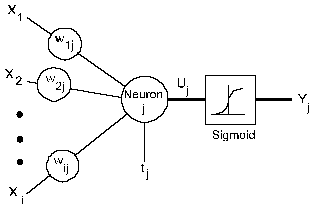
\includegraphics[scale=.3, angle=0]{Files/nn2.png}
    \caption[Single-layer Neural Networks (Perceptrons)]{Single-layer Neural Networks (Perceptrons)}
    \label{fig:NNNN}
\end{figure}


\par
Now that we are clear with the definition, we now explain fully feed forward neural network.
\section{Feed Forward Neural Network}
The feed forward neural network is an extension of the above concept. It consists of multiple layers, each layer has multiple neurons and information flows from input to the output. Important characteristics of a feed forward neural network is of not having any loop. Intuitively, feed forward neural network is a digraph containing neurons as nodes and weighted edges. To train a feed forward neural network the most popular technique is backpropagation.
\begin{figure}[H]
  \centering
    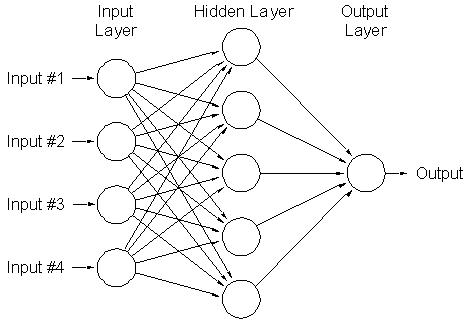
\includegraphics[scale=.6, angle=0]{Files/FFNN.png}
    \caption[Feed Forward Neural Network]{Feed Forward Neural Network}
    \label{fig:FFNN}
\end{figure}

\section{Backpropagation}
 Backprogation\cite{rumelhart1988learning} is an algorithm to find the local minima of an error function. In a feed forward neural network we have neurons and edges with weights which need to be fined tuned based on the output and error function.  The backpropagation algorithm computes the loss and uses  optimization algorithms such as gradient descent to propagate error in the backward direction recursively. This causes the change in weights of the edges which enables the whole network to adapt according to the data.  
\begin{figure}[H]
  \centering
    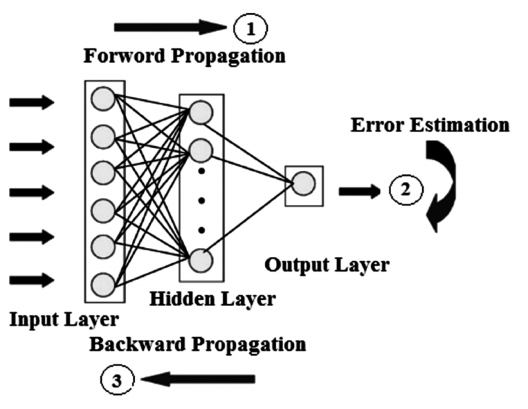
\includegraphics[scale=.4, angle=0]{Files/BackPropagation.png}
    \caption[Back Propagation Visualization]{Back Propagation Visualization}
    \label{fig:FFNN}
\end{figure}

\section{Convolution Neural Network}

Convolution Neural Network are a variant of multi layer perceptron. inspired by the organization of the animal visual cortex. Convolution Neural Networks have repetitive blocks of neurons also known as features or kernels extending across the space. These repetitive blocks share weights during training. The CNN contains various types of layers, out of which the important layers are  as follows:

\subsection{Convolution}

Convolution is mathematical operation applied over two real valued arguments. Suppose we have two functions $f(x)$ and $h(x)$, then convolution operation over one dimension would be 

 \begin{equation}\label{eq:convolution-1d}
        \begin{aligned}
            g(x)=f(x) \ast h(x) = \int_{-\infty }^{\infty} f(s) \times h(x-s) ds
        \end{aligned}
\end{equation}

Here s is dummy integration variable. 
From the CNN and image perspective, our image becomes f(x) and kernel or feature map becomes h(x). The feature map is slided across the image and as it slides we apply the convolution operation over it to generate the output feature map. The values of these filters are fine tuned during training, but we have to decide the following key parameters commonly known as hyper-parameters before training.
\begin{itemize}
    \item  Depth corresponds to the number of filters or kernels mapped at any layer. In the \cref{fig:CNN} we can see that first layer we have 4 feature maps.
    \item Stride corresponds to the number of steps we take when we slide a feature map over the ouput from previous layer. For example, when we have set stride as 1 the, we slide filter on step and when we have set the stride as 3 the we slide the filter 3 steps each time.
\end{itemize}

\subsection{ Activation function}
Once convolution operation has been performed we apply a non linear activation function such as tanh, RELU, leakyRELU.

\subsection{Pooling}
Pooling is basically reducing the dimension space as it get increased by adding various feature maps. To reduce the dimension, there are various kinds of pooling function such as max, add, min. Here based on value of receptive field, the pooling operation is performed over the feature map obtained from the previous layer. For example, for a receptive field of value 2 and pooling function as max, we take a max value from every $2 \times 2$ area of feature map.


\subsection{Fully Connected layer}
The last output layer is a fully connected layer over which various cost function such as sigmoid, soft-max are applied to generate the output.


\begin{figure}[H]
  \centering
    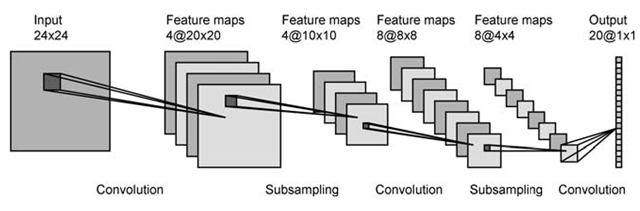
\includegraphics[scale=.6, angle=0]{Files/cnn-2.png}
    \caption[Convolutional Neural Network]{Convolutional Neural Network}
    \label{fig:CNN}
\end{figure} % Experimental Setup

\chap{Enhanced Generative Adversarial Network}

\section{Introduction}
The original GAN as we discussed in the previous chapters suffered from various issues such s model collapse, convergence issue. There have been many variation which have come up. In this chapter we discuss the architecture and methodologies which we have adopted in our work.  


\section{GAN Architecture} 

The original paper's\cite{Original-GAN} generator architecture consisted of  rectifier linear\cite{RELU} and sigmoid activations, while the discriminator net used maxout [10] activations. the results were good but lacked stability and also suffered from the problem of model collapse.
Later, Radford \textit{et al.}\cite{DCGAN} proposed deep convolution generative adversarial network which used deep convolution with fractional stride convolution and batch normalization to stabilize the model. This work uses this architecture as base and later adding conditional vector to it. The figure 4.1 shows the architecture of generator and discriminator. In this work, we use RELU
in all the layers expect the output. Since the paper Radford \textit{et al.}\cite{DCGAN} showed that these can help in convergence of the model and it also covers the color space of the distribution.
\par

As you can see it figure the architecture of generator and discriminatory are exactly opposite to each other. The generator uses up-convolution or commonly known as backward convolution to generate image.%J. Long, E. Shelhamer, and T. Darrell, “Fully convolutional networks for semantic segmentation,”CoRR, vol. abs/1411.4038, 2014. [Online]. Available: http://arxiv.org/abs/1411.4038
The discriminator is a standard deep convolution neural network used for classification of real or  a fake image.
\begin{figure}
  \centering
    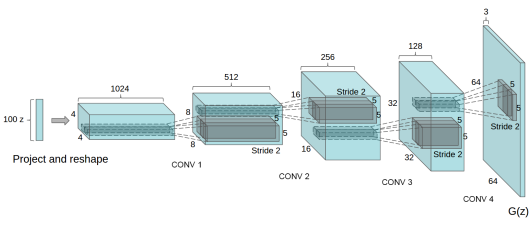
\includegraphics[scale=.7, angle=0]{Files/Generator-Architecture.png}
    \caption[Generator Architecture]{Generator Architecture\cite{DCGAN}}
    \label{fig: DCGAN}
\end{figure}

\section{Training GAN}

Training a GAN is always a tricky part. This work uses DCGAN\cite{DCGAN} as baseline, as the DCGAN has shown that it can stabilizes the networks to a great extent. The major contribution of the DCGAN in our work is the use of Batch-Normalization, strided convolution and ADAM optimizer. We will go through each of these steps one by one.
\subsection{BatchNomalization}

Batch Normalization was first introduced by Ioffe \textit{et al.}\cite{BatchNorm}. It is a major landmark in area of deep learning as most of the current deep neural network frameworks contains batch normalization. 
To understand batch normalization, we need to understand the problem it is trying to solve. Its major aim is to minimize internal co-variance shift. Internal covariance shift refers to the change in input distribution as we are feeding data in mini batches. Since a neural network are designed in hierarchical fashion, even small change in form of an outlier can get amplified as we are dealing with generally more than a million parameters and several layers. To rectify this problem, we normalize each batch at every layer, by both mean and variance. This process is commonly called as whitning. The major advantages of the batch normalization are as follows.
\begin{itemize}
    \item Initial value of weights have less impact on gradient descent.
    \item It helps in keeping higher learning rate and accuracy. Hence it reduces overall training time and this helps in faster training of the GANs.
\end{itemize}

\subsection{Strided Convolution}

The concept of deconvolution was first introduced by Zeiler \textit{et al} \cite{Deconv}. It also is commonly known as  strided convolution, transposed fractional convolution or upsampling.



\par
It is basically going from output of some convolution to the input to that convolution. For instance, it is going from the green matrix to the blue matrix as shown in the below figure. So given a kernel K, the type of convolution is defined by how forward or backward passes are calculated\cite{Deconv-Theano}.


\begin{figure}[ht]
  \centering
    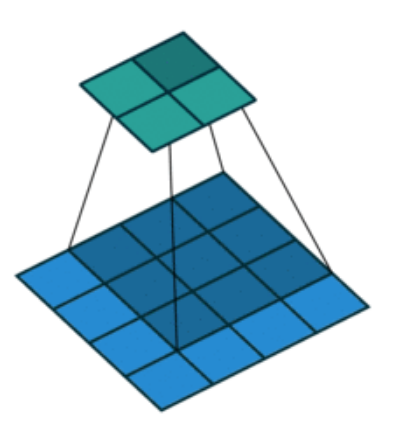
\includegraphics[scale=.5, angle=0]{Files/simple-conv.png}
    \caption[Simple Convolution]{Simple Convolution \cite{Deconv-Theano}}
    \label{fig: Simple Convolution}
\end{figure}

\begin{figure}[ht]
  \centering
    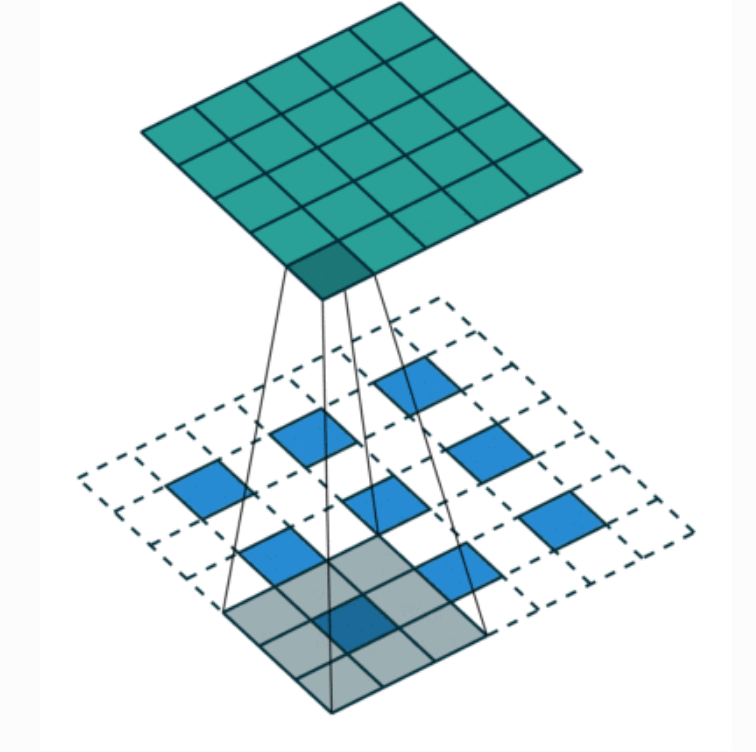
\includegraphics[scale=.4, angle=0]{Files/Frational-Stride-Conv.png}
    \caption[Transpose Convolution ]{Transpose Convolution \cite{Deconv-Theano}}
    \label{fig: Strided Convolution}
\end{figure}



\subsection{ADAM Optimizer}

Adaptive Moment Estimation whihc more commontly known as ADAM optimizer is a stochastic gradient descent(SGD) optimizer. It was first proposed by Diederik \textit{et al.} \cite{Adam}. The vanilla stochastic gradient descent suffers from many problems. But the three key issues which directly related to our work are as follows.
\begin{itemize}
    \item In case of non convex error function, the neural network can be stuck at non local optima.
    \item Choosing correct learning is always a challenging task and it can cause longer time for SGD algorithm to converge.
    \item Specifically in our work, where we are trying to model the data and it is sparse. Vanilla SGD doesn't provide flexibility for having different learning rate for each weight.

To overcome this problem we use ADAM optimizer in our work. It combines adagrade\cite{Adagrade} and momentum-optimizer \cite{momentum}. It 

\end{itemize}
 
 
  % Experiment 1

%\chap{Experiments and Results}


\section{Introduction}

In this chapter, we look at the implementation perspective of the whole system. We look at the three datasets we used and the results obtained from them. We later compare the results with the existing implementations and the application of this model over various domains. 


\section{DataSet}
\subsection{MNIST}
\subsection{CelebA}
\subsection{CIFAR-10}

\section{System Design}



 % Experiment 2

%\doublespacing
\chap{Experiments and Results}
\label{chap:EnR}

\section{Introduction}

In this chapter, we look at the implementation perspective of the whole system. We also look at the three dataset we used and the results obtained from them. 

\section{Implementation Details}
To implement the conditional generative adversarial network we used Tensorflow\cite{tensorflow2015-whitepaper} with Kera\cite{keras}. The structure of generator and discriminator are described in \cref{Generator-Activation} and \cref{Discriminator-Table}.
\begin{table}[ht]
\centering
\caption{Generator Architecture Specification}
\label{Generator-Activation}
\begin{tabular}{llll}
Operation       & Stride & Features & Activation \\
Merge Input     & -      & -        & -          \\
Dense layer     & -      & -        & Sigmoid    \\
Deconvolution 1 & 5 * 5  & 512      & RELU       \\
Deconvolution 2 & 5 * 5    & 256      & RELU       \\
Deconvolution 3 & 5 * 5   & 128      & RELU       \\
Deconvolution 4 & 5 * 5   & 64       & RELU       \\
Deconvolution 5 & 5 * 5  & 3        & Tanh      
\end{tabular}
\end{table}
\begin{table}[ht]
\centering
\caption{Discriminator Architecture Specification}
\label{Discriminator-Table}
\begin{tabular}{llll}
Operation     & Stride & Features & Activation \\
Convolution 1 & 5 * 5  & 64       & Leaky RELU \\
Convolution 2 & 5*5    & 128      & LeakyRELU  \\
Convolution 3 & 5 *5   & 256      & LeakyRELU  \\
Convolution 4 & 5 *5   & 512      & LeakyRELU  \\
Convolution 5 & 5 * 5  & 1        & Softmax    \\
Convolution 5 & 5*5    & 18       & Sigmoid   
\end{tabular}
\end{table}
\section{Training}
Since the discriminator was weak, before actual training we trained the discriminator in two steps. Firstly we added a conditional vector to its input and removed the classification output of it. And then we trained the discriminator with real images with incorrect label to classify as fake image. Secondly, to the original discriminator we copied the weights from the previous training and trained again on real images to classify the them into the particular class.  


In the below figure we can look at the training losses for the generator and the discriminator. As we can observe after pre-training a GAN, we are able to reach a equilibrium loss for both generator and discriminator at around epoch 30. If we also look at graph closely, in starting epoch the generator and discriminator have a huge loss gap as we are playing minmax game. 

\begin{figure}[H]
  \centering
    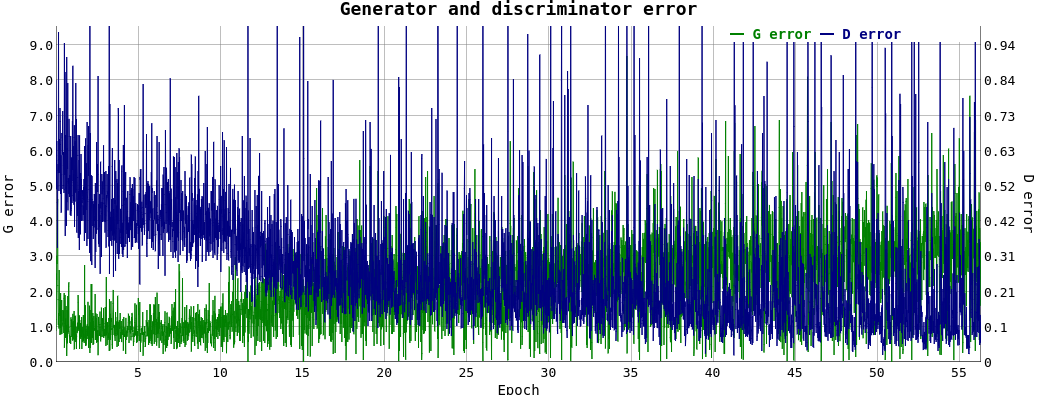
\includegraphics[scale=.4, angle=0]{Files/Training-2.png}
    \caption[Generator Discrminator Loss for Celeba dataset]{}
    \label{fig:train-celeba}
\end{figure}

\begin{figure}[H]
  \centering
    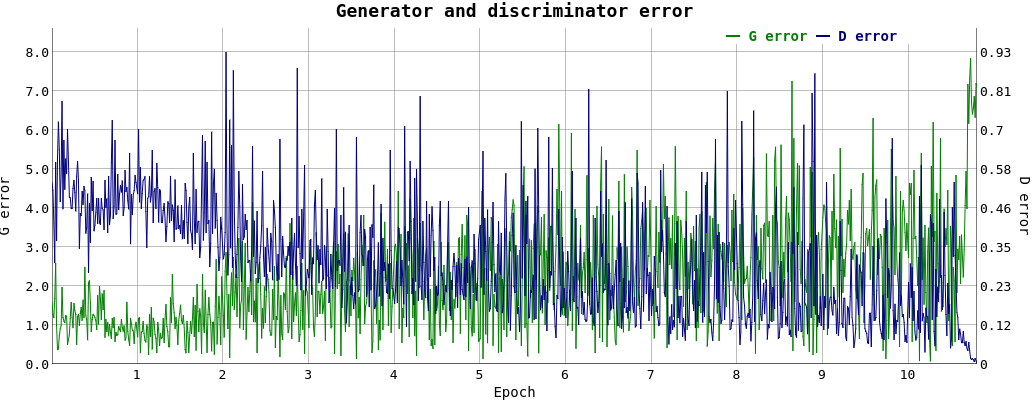
\includegraphics[scale=.4, angle=0]{Files/MNIST-GAN.png}
    \caption[Generator Discrminator Loss for MNIST dataset]{}
    \label{fig:train-mnist}
\end{figure}
\section{DataSet}
\subsection{CelebA}
The CelebFaces Attributes dataset (CelebA)\cite{celeba} contains 202599 face images of celebrities. As some of the categories are very less , so we removed certain categories from our training. . The sdistribution of the overall dataset is shown in \cref{fig:celeba}. As part of preprocessing, we crop the images to $64 \times 64$.The reason for cropping the images is to focus on faces in the images and as they are already aligned.


\begin{figure}[H]
  \centering
    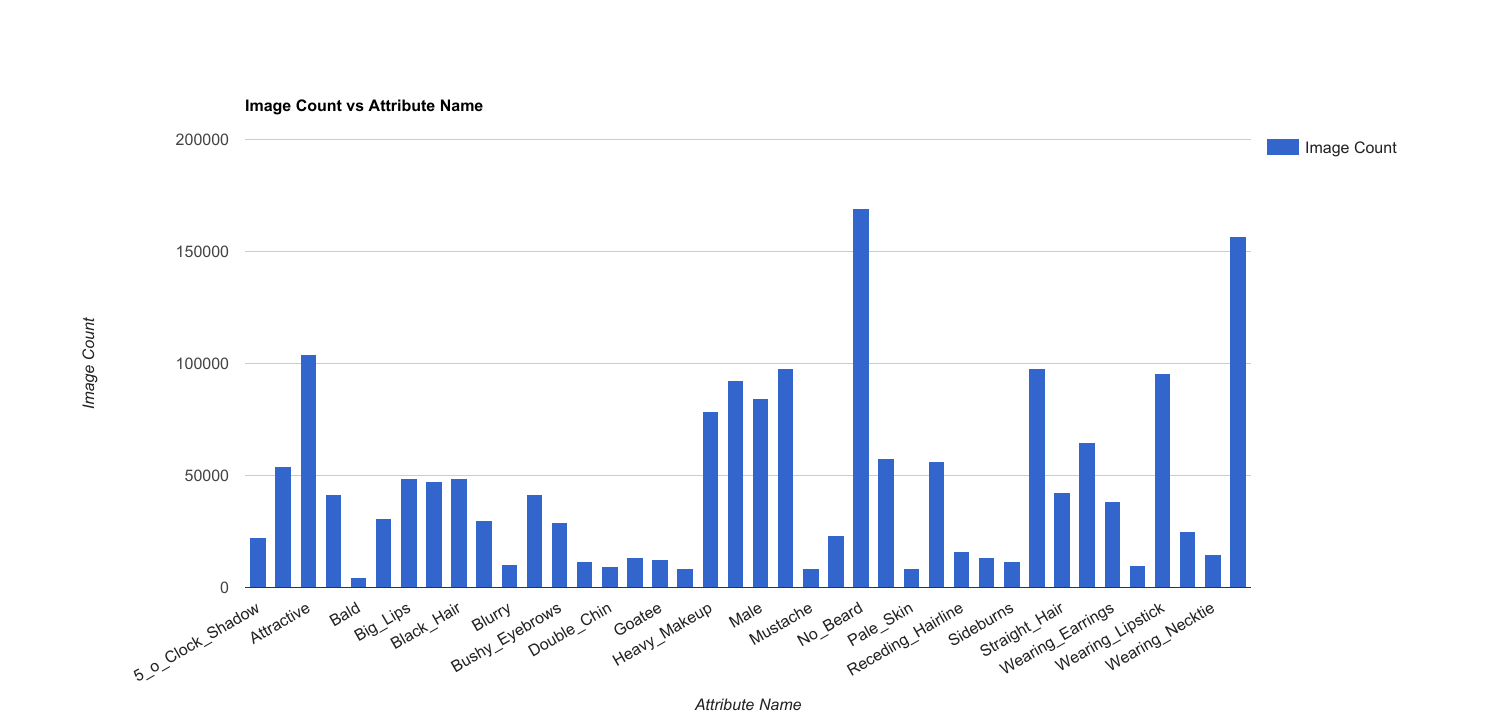
\includegraphics[scale=.3, angle=0]{Files/celeba-visualize.png}
    \caption[Generator Architecture]{Generator Architecture\cite{DCGAN}}
    \label{fig:celeba}
\end{figure}
%\subsection{CIFAR-10}

\subsection{MNIST}
The MNIST dataset is very standard image processing dataset. This dataset contains 60000 labeled images of digits from 0 to 9. This dataset helps in validating the models correctness in very short time. Since neural  network take lot of time to converge, so if we have some issue with our implementation or logic then we can debug in very short amount of time using this dataset.

\section{Results}

Once the generator has been trained, we look at the images being generated by our generator. by passing some random noise(z) along with the conditional vector. We can see in \cref{Celeb-a} the various different category facial images being drawn by our generator. There were several categories as shown in \cref{U-celeb-a} for which generator was unsuccessful in getting desired facial attributes. Similarly, we generated different kind of digits from the MNIST trained generator as shown in \cref{MNIST-Result}. Since MNIST dataset does not involve any complexity, hence there were very less unsuccessful result when generating specific digits.

  

\begin{table}[ht]
\centering
\caption{Successfully Generated Celebrity Images}
\label{Celeb-a}
\begin{tabular}{|llllll|}
\hline
Bald & 
\includegraphics[width=1.69cm, height=1.69cm]{Files/images/images1/image100.png}  &
\includegraphics[width=1.69cm, height=1.69cm]{Files/images/images1/image2.png}   & 
\includegraphics[width=1.69cm, height=1.69cm]{Files/images/images1/image3.png}  & 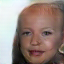
\includegraphics[width=1.69cm, height=1.69cm]{Files/images/images1/image52.png}  & 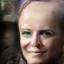
\includegraphics[width=1.69cm, height=1.69cm]{Files/images/images1/image68.png} \\ \hline


Bangs & 
\includegraphics[width=1.69cm, height=1.69cm]{Files/images/images2/image74.png}  &
\includegraphics[width=1.69cm, height=1.69cm]{Files/images/images2/image9.png}   & 
\includegraphics[width=1.69cm, height=1.69cm]{Files/images/images2/image77.png}  & 
\includegraphics[width=1.69cm, height=1.69cm]{Files/images/images2/image79.png}  & 
\includegraphics[width=1.69cm, height=1.69cm]{Files/images/images2/image48.png} \\ \hline


Black Hair & 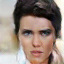
\includegraphics[width=1.69cm, height=1.69cm]{Files/images/images3/image94.png}  &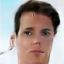
\includegraphics[width=1.69cm, height=1.69cm]{Files/images/images3/image60.png}   & 
\includegraphics[width=1.69cm, height=1.69cm]{Files/images/images3/image56.png}  & 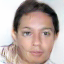
\includegraphics[width=1.69cm, height=1.69cm]{Files/images/images3/image87.png}  & 
\includegraphics[width=1.69cm, height=1.69cm]{Files/images/images3/image76.png} \\ \hline


Blond & 
\includegraphics[width=1.69cm, height=1.69cm]{Files/images/images4/image86.png}  &
\includegraphics[width=1.69cm, height=1.69cm]{Files/images/images4/image64.png}   & 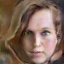
\includegraphics[width=1.69cm, height=1.69cm]{Files/images/images4/image91.png}  & 
\includegraphics[width=1.69cm, height=1.69cm]{Files/images/images4/image5.png}  & 
\includegraphics[width=1.69cm, height=1.69cm]{Files/images/images4/image25.png} \\ \hline


Male & 
\includegraphics[width=1.69cm, height=1.69cm]{Files/images/images10/image12.png}  &
\includegraphics[width=1.69cm, height=1.69cm]{Files/images/images10/image32.png}   & 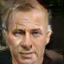
\includegraphics[width=1.69cm, height=1.69cm]{Files/images/images10/image19.png}  & 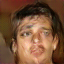
\includegraphics[width=1.69cm, height=1.69cm]{Files/images/images10/image34.png}  & 
\includegraphics[width=1.69cm, height=1.69cm]{Files/images/images10/image55.png} \\ \hline

Mouth Open  & 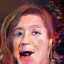
\includegraphics[width=1.69cm, height=1.69cm]{Files/images/images11/image70.png}  &
\includegraphics[width=1.69cm, height=1.69cm]{Files/images/images11/image69.png}   & 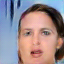
\includegraphics[width=1.69cm, height=1.69cm]{Files/images/images11/image65.png}  & 
\includegraphics[width=1.69cm, height=1.69cm]{Files/images/images11/image37.png}  & 
\includegraphics[width=1.69cm, height=1.69cm]{Files/images/images11/image7.png} \\ \hline

Smiling  & 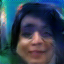
\includegraphics[width=1.69cm, height=1.69cm]{Files/images/images15/image70.png}  &
\includegraphics[width=1.69cm, height=1.69cm]{Files/images/images15/image7.png}   & 
\includegraphics[width=1.69cm, height=1.69cm]{Files/images/images15/image47.png}  & 
\includegraphics[width=1.69cm, height=1.69cm]{Files/images/images15/image37.png}  & 
\includegraphics[width=1.69cm, height=1.69cm]{Files/images/images15/image76.png} \\ \hline

Eye Glasses  & 
\includegraphics[width=1.69cm, height=1.69cm]{Files/images/images7/image79.png}  &
\includegraphics[width=1.69cm, height=1.69cm]{Files/images/images7/image4.png}   & 
\includegraphics[width=1.69cm, height=1.69cm]{Files/images/images7/image27.png}  & 
\includegraphics[width=1.69cm, height=1.69cm]{Files/images/images7/image25.png}  & 
\includegraphics[width=1.69cm, height=1.69cm]{Files/images/images7/image67.png} \\ \hline

Eye Glasses  & \includegraphics[width=1.69cm, height=1.69cm]{Files/images/images7/image79.png}  &\includegraphics[width=1.69cm, height=1.69cm]{Files/images/images7/image4.png}   & \includegraphics[width=1.69cm, height=1.69cm]{Files/images/images7/image27.png}  & \includegraphics[width=1.69cm, height=1.69cm]{Files/images/images7/image25.png}  & \includegraphics[width=1.69cm, height=1.69cm]{Files/images/images7/image67.png} \\ \hline
\end{tabular}
\end{table}

\begin{table}[H]
\centering
\caption{Unsuccessful Generated Celebrity Images}
\label{U-celeb-a}
\begin{tabular}{|llllll|}
\hline
Wearing Hat & \includegraphics[width=1.69cm, height=1.69cm]{Files/images/images18/image1.png}  &\includegraphics[width=1.69cm, height=1.69cm]{Files/images/images18/image2.png}   & \includegraphics[width=1.69cm, height=1.69cm]{Files/images/images18/image3.png}  & \includegraphics[width=1.69cm, height=1.69cm]{Files/images/images18/image52.png}  & \includegraphics[width=1.69cm, height=1.69cm]{Files/images/images18/image68.png} \\ \hline


Wavy Hair & \includegraphics[width=1.69cm, height=1.69cm]{Files/images/images17/image1.png}  &\includegraphics[width=1.69cm, height=1.69cm]{Files/images/images17/image2.png}   & \includegraphics[width=1.69cm, height=1.69cm]{Files/images/images17/image3.png}  & \includegraphics[width=1.69cm, height=1.69cm]{Files/images/images17/image52.png}  & \includegraphics[width=1.69cm, height=1.69cm]{Files/images/images17/image68.png} \\ \hline

Receding Hairline & \includegraphics[width=1.69cm, height=1.69cm]{Files/images/images14/image1.png}  &\includegraphics[width=1.69cm, height=1.69cm]{Files/images/images14/image2.png}   & \includegraphics[width=1.69cm, height=1.69cm]{Files/images/images14/image3.png}  & \includegraphics[width=1.69cm, height=1.69cm]{Files/images/images14/image52.png}  & \includegraphics[width=1.69cm, height=1.69cm]{Files/images/images14/image68.png} \\ \hline


\end{tabular}
\end{table}

\begin{table}[H]
\centering
\caption{Successfully Generated MNIST Images}
\label{MNIST-Result}
\begin{tabular}{|llllll|}
\hline
0 & \includegraphics[width=1.69cm, height=1.69cm]{Files/MNIST/0-0.png}  &\includegraphics[width=1.69cm,  height=1.69cm]{Files/MNIST/1-2.png}   & \includegraphics[width=1.69cm, height=1.69cm]{Files/MNIST/2-4.png}  & \includegraphics[width=1.69cm, height=1.69cm]{Files/MNIST/5-0.png}  & \includegraphics[width=1.69cm, height=1.69cm]{Files/MNIST/6-2.png} \\ \hline

1 & \includegraphics[width=1.69cm, height=1.69cm]{Files/MNIST/0-1.png}  &\includegraphics[width=1.69cm, height=1.69cm]{Files/MNIST/1-3.png}   & \includegraphics[width=1.69cm, height=1.69cm]{Files/MNIST/2-5.png}  & \includegraphics[width=1.69cm, height=1.69cm]{Files/MNIST/5-1.png}  & \includegraphics[width=1.69cm, height=1.69cm]{Files/MNIST/7-5.png} \\ \hline

2 & \includegraphics[width=1.69cm, height=1.69cm]{Files/MNIST/0-2.png}  &\includegraphics[width=1.69cm, height=1.69cm]{Files/MNIST/1-4.png}   & \includegraphics[width=1.69cm, height=1.69cm]{Files/MNIST/2-6.png}  & \includegraphics[width=1.69cm, height=1.69cm]{Files/MNIST/5-2.png}  & \includegraphics[width=1.69cm, height=1.69cm]{Files/MNIST/6-4.png} \\ \hline

3 & \includegraphics[width=1.69cm, height=1.69cm]{Files/MNIST/0-3.png}  &\includegraphics[width=1.69cm, height=1.69cm]{Files/MNIST/1-5.png}   & \includegraphics[width=1.69cm, height=1.69cm]{Files/MNIST/2-7.png}  & \includegraphics[width=1.69cm, height=1.69cm]{Files/MNIST/5-3.png}  & \includegraphics[width=1.69cm, height=1.69cm]{Files/MNIST/6-5.png} \\ \hline

4 & \includegraphics[width=1.69cm, height=1.69cm]{Files/MNIST/0-4.png}  &\includegraphics[width=1.69cm, height=1.69cm]{Files/MNIST/1-6.png}   & \includegraphics[width=1.69cm, height=1.69cm]{Files/MNIST/3-0.png}  & \includegraphics[width=1.69cm, height=1.69cm]{Files/MNIST/5-4.png}  & \includegraphics[width=1.69cm, height=1.69cm]{Files/MNIST/6-6.png} \\ \hline

5 & \includegraphics[width=1.69cm, height=1.69cm]{Files/MNIST/0-5.png}  &\includegraphics[width=1.69cm, height=1.69cm]{Files/MNIST/1-7.png}   & \includegraphics[width=1.69cm, height=1.69cm]{Files/MNIST/3-1.png}  & \includegraphics[width=1.69cm, height=1.69cm]{Files/MNIST/5-5.png}  & \includegraphics[width=1.69cm, height=1.69cm]{Files/MNIST/6-7.png} \\ \hline

6 & \includegraphics[width=1.69cm, height=1.69cm]{Files/MNIST/0-6.png}  &\includegraphics[width=1.69cm, height=1.69cm]{Files/MNIST/2-0.png}   & \includegraphics[width=1.69cm, height=1.69cm]{Files/MNIST/3-2.png}  & \includegraphics[width=1.69cm, height=1.69cm]{Files/MNIST/5-6.png}  & \includegraphics[width=1.69cm, height=1.69cm]{Files/MNIST/7-0.png} \\ \hline

7 & \includegraphics[width=1.69cm, height=1.69cm]{Files/MNIST/0-7.png}  &\includegraphics[width=1.69cm, height=1.69cm]{Files/MNIST/2-1.png}   & \includegraphics[width=1.69cm, height=1.69cm]{Files/MNIST/3-3.png}  & \includegraphics[width=1.69cm, height=1.69cm]{Files/MNIST/4-5.png}  & \includegraphics[width=1.69cm, height=1.69cm]{Files/MNIST/5-7.png} \\ \hline

8 & \includegraphics[width=1.69cm, height=1.69cm]{Files/MNIST/1-0.png}  &\includegraphics[width=1.69cm, height=1.69cm]{Files/MNIST/2-2.png}   & \includegraphics[width=1.69cm, height=1.69cm]{Files/MNIST/3-4.png}  & \includegraphics[width=1.69cm, height=1.69cm]{Files/MNIST/4-6.png}  & \includegraphics[width=1.69cm, height=1.69cm]{Files/MNIST/7-2.png} \\ \hline

9 & \includegraphics[width=1.69cm, height=1.69cm]{Files/MNIST/1-1.png}  &\includegraphics[width=1.69cm, height=1.69cm]{Files/MNIST/2-3.png}   & \includegraphics[width=1.69cm, height=1.69cm]{Files/MNIST/4-7.png}  & \includegraphics[width=1.69cm, height=1.69cm]{Files/MNIST/6-1.png}  & \includegraphics[width=1.69cm, height=1.69cm]{Files/MNIST/7-3.png} \\ \hline

\end{tabular}
\end{table}



\section{Evaluation}

It is very challenging to evaluate the performance of GAN networks as there has been no comparable method to judge the quality of images being produced.  To evaluate the performance of celebA \cite{celeba} dataset , we use the same discriminator and we train it over the real images dataset. Later we passed 100 generated images from each category to this CNN to obtain a mean accuracy of 85.23\%. We also ran text over Microsoft's Vision API \cite{Microsoft}, where we passed 1000 facial images for which it was able to detect faces with 96.88\%.  % Results and Discussion

%\doublespacing
\chap{Conclusion}
\label{chap:Conclusion}

The main aim of this work to carefully study, understand, document the generative adversarial network from ground up. We start with understanding the  convolutional neural network as it is one the major component of this work. In \autoref{chap:CNN} we study 101 of CNNs. Later in \autoref{chap:RelatedWork}, we look at the previous generation models. Since the GAN are currently a hot topic in field of depp learning and computer vision. This can be seen from many framework being proposed in recent years and we look at some of them in \autoref{chap:RelatedWork}. By looking at some of the work we started with conditional generation of the image as this is one of the key sub-problem for many large problem such as generating images from caption, generating complex captcha. In \autoref{chap:EGAN} we take propose the  tweaks and tricks that many authors failed to mention in their research. During experimentation phase we faced lot of challenges in producing any kind of images but with techniques proposed in \autoref{chap:EnR} we proposed some approaches we took train the network in very less epochs.
\par
In the end, there is still a long way to have a stabilized and reliable method for generating images using GAN. There is also need for a better way to quantify the  performance of a GAN framework. % Conclusion



%% Appendices -----------------------------------------------------
%\addtocontents{toc}{\vspace{2em}} % Add a gap in the Contents, for aesthetics
%\lhead{\emph{Appendices}}  % Change the left side page header to "Appendices"
%\appendix % Cue to tell LaTeX that the following 'chapters' are Appendices

%\chap{An Appendix}

Lorem ipsum dolor sit amet, consectetur adipiscing elit. Vivamus at pulvinar nisi. Phasellus hendrerit, diam placerat interdum iaculis, mauris justo cursus risus, in viverra purus eros at ligula. Ut metus justo, consequat a tristique posuere, laoreet nec nibh. Etiam et scelerisque mauris. Phasellus vel massa magna. Ut non neque id tortor pharetra bibendum vitae sit amet nisi. Duis nec quam quam, sed euismod justo. Pellentesque eu tellus vitae ante tempus malesuada. Nunc accumsan, quam in congue consequat, lectus lectus dapibus erat, id aliquet urna neque at massa. Nulla facilisi. Morbi ullamcorper eleifend posuere. Donec libero leo, faucibus nec bibendum at, mattis et urna. Proin consectetur, nunc ut imperdiet lobortis, magna neque tincidunt lectus, id iaculis nisi justo id nibh. Pellentesque vel sem in erat vulputate faucibus molestie ut lorem.

Quisque tristique urna in lorem laoreet at laoreet quam congue. Donec dolor turpis, blandit non imperdiet aliquet, blandit et felis. In lorem nisi, pretium sit amet vestibulum sed, tempus et sem. Proin non ante turpis. Nulla imperdiet fringilla convallis. Vivamus vel bibendum nisl. Pellentesque justo lectus, molestie vel luctus sed, lobortis in libero. Nulla facilisi. Aliquam erat volutpat. Suspendisse vitae nunc nunc. Sed aliquet est suscipit sapien rhoncus non adipiscing nibh consequat. Aliquam metus urna, faucibus eu vulputate non, luctus eu justo.

Donec urna leo, vulputate vitae porta eu, vehicula blandit libero. Phasellus eget massa et leo condimentum mollis. Nullam molestie, justo at pellentesque vulputate, sapien velit ornare diam, nec gravida lacus augue non diam. Integer mattis lacus id libero ultrices sit amet mollis neque molestie. Integer ut leo eget mi volutpat congue. Vivamus sodales, turpis id venenatis placerat, tellus purus adipiscing magna, eu aliquam nibh dolor id nibh. Pellentesque habitant morbi tristique senectus et netus et malesuada fames ac turpis egestas. Sed cursus convallis quam nec vehicula. Sed vulputate neque eget odio fringilla ac sodales urna feugiat.

Phasellus nisi quam, volutpat non ullamcorper eget, congue fringilla leo. Cras et erat et nibh placerat commodo id ornare est. Nulla facilisi. Aenean pulvinar scelerisque eros eget interdum. Nunc pulvinar magna ut felis varius in hendrerit dolor accumsan. Nunc pellentesque magna quis magna bibendum non laoreet erat tincidunt. Nulla facilisi.

Duis eget massa sem, gravida interdum ipsum. Nulla nunc nisl, hendrerit sit amet commodo vel, varius id tellus. Lorem ipsum dolor sit amet, consectetur adipiscing elit. Nunc ac dolor est. Suspendisse ultrices tincidunt metus eget accumsan. Nullam facilisis, justo vitae convallis sollicitudin, eros augue malesuada metus, nec sagittis diam nibh ut sapien. Duis blandit lectus vitae lorem aliquam nec euismod nisi volutpat. Vestibulum ornare dictum tortor, at faucibus justo tempor non. Nulla facilisi. Cras non massa nunc, eget euismod purus. Nunc metus ipsum, euismod a consectetur vel, hendrerit nec nunc. % Appendix Title

%\input{Appendices/AppendixB} % Appendix Title

%\input{Appendices/AppendixC} % Appendix Title


%% Bibliography ---------------------------------------------------
\backmatter % Cue to tell LaTeX that the following 'chapters' are Bibliography
\label{Bibliography}
\lhead{\emph{Bibliography}}  % left side page header to "Bibliography"
\bibliographystyle{plain}  % Use the "unsrtnat" BibTeX style for formatting the Bibliography

\begingroup
    \raggedright
    \sloppy
    \bibliography{Bibliography}  % The references (bibliography) information are stored in the file named "Bibliography.bib"
\endgroup 


\end{document}  % The End
%% ----------------------------------------------------------------